% Estimating viewpoint continuously to fine tune a initial matching
The NZ-WHO template matching method we have presented
(Sect.~\ref{sec:nzwho}) makes template generation and evaluation
computationally inexpensive. This means that we can use a
hypothesize-and-test scheme to efficiently explore the continuous
parameter space to find the best object pose, scale, 3D CAD model type
and camera focal length.
%
In particular, we propose to implement this parameter search as a
Markov Chain Monte Carlo (MCMC) procedure based on the
Metropolis-Hastings algorithm.

\paragraph{Probabilistic formulation.}
We parameterize the continuous parameter space as  $p = [v, m, f]$,
where $v$ is the 3D rotation of the CAD model, $m$ is the discrete CAD
model index, and $f$ is the focal length.

We model the probability that the object in the test image
$\mathcal{I}$ is generated by the parameters $p$ as a distribution in
the exponential family, and let
\begin{align}
    P(p) & \sim e^{ \max_{s} w(p) \ast \mathcal{T}_s(\mathcal{I})},
\end{align}
where $\max_{s} w(p) \ast T_s(\mathcal{I})$ is the maximum convolution score of
NZ-WHO template $w(p)$ with image features $T_s(\mathcal{I})$ for all scale $s$, as defined
in Sect.~\ref{sec:nzwho}. 

\paragraph{Inference.}
We approximate the MAP solution for $p$ by drawing samples from the
distribution $P(p)$, using the single component Metropolis-Hastings
algorithm. Specifically, we use a variant that changes only a single
component of the parameter vector $p$ at a time, termed Single
Component Metropolis Hastings \cite{mcmc}.

This algorithm changes the current state $p$ to a new state $q$ based
on the acceptance probability
\begin{align}
    A(p \rightarrow q) & =  min\left( 1,  \frac{P(q) g(q \rightarrow p)}{P(p) g(p \rightarrow q)}\right).
\end{align}
We define $3$ different types of moves that can alter the state
(Fig.~\ref{fig:moves}), {\em (i)} changing the focal length $f$, {\em
(ii)} one of the rotational pose parameters $v_i$, and {\em (iii)} CAD model
index $m$. For (i) and (ii), we use Gaussian proposal distributions, and a uniform
distribution over model changes for (iii). For scale and translation, we
implicitly compute all possible translation and scale by convolving $w(q)$ to
HOG pyramid.
\begin{align}
    g(p \rightarrow p + v_i') & \sim \mathcal{N}(\mu = p_{v_i},\sigma = \sigma_v) \quad i \in \{1,2,3\}\\
    g(p \rightarrow p + f') & \sim \mathcal{N}(\mu = p_{f},\sigma = \sigma_f)\\
    g(p \rightarrow p + m') & \sim c \delta(p_m) + (1-c) Unif(1,M),
\end{align}
where $g$ is the proposal distribution. % and $P$ is the distribution of which we
%defined using Gaussian distribution around previous state. $A$ is the
%acceptance probability where we accept new proposal with $A(x \rightarrow x')$.
%
% One can also think of the image as an image cropped by detection
% bounding box. We synthesize covariance matrix and create NZ-WHO
% template $w(x)$ for particular viewpoint, focal length and CAD model.
% In sum, for new proposal $x'$, we make a NZ-WHO template on the fly 
% We found out that it requires good initialization to converge to
% local minima.

In practice, we run this algorithm for 20 iterations, keeping
the sample with the highest probability as our approximate estimate of
the MAP solution. We set $\sigma_v = 5$ degree and $\sigma_f = 1$ and
$c = 0.1$ for all experiments.

% there are several advantages that was not possible such as
% \textbf{on-the-fly} template generation and making large number of
% templates
\begin{figure}[t]
\centering
    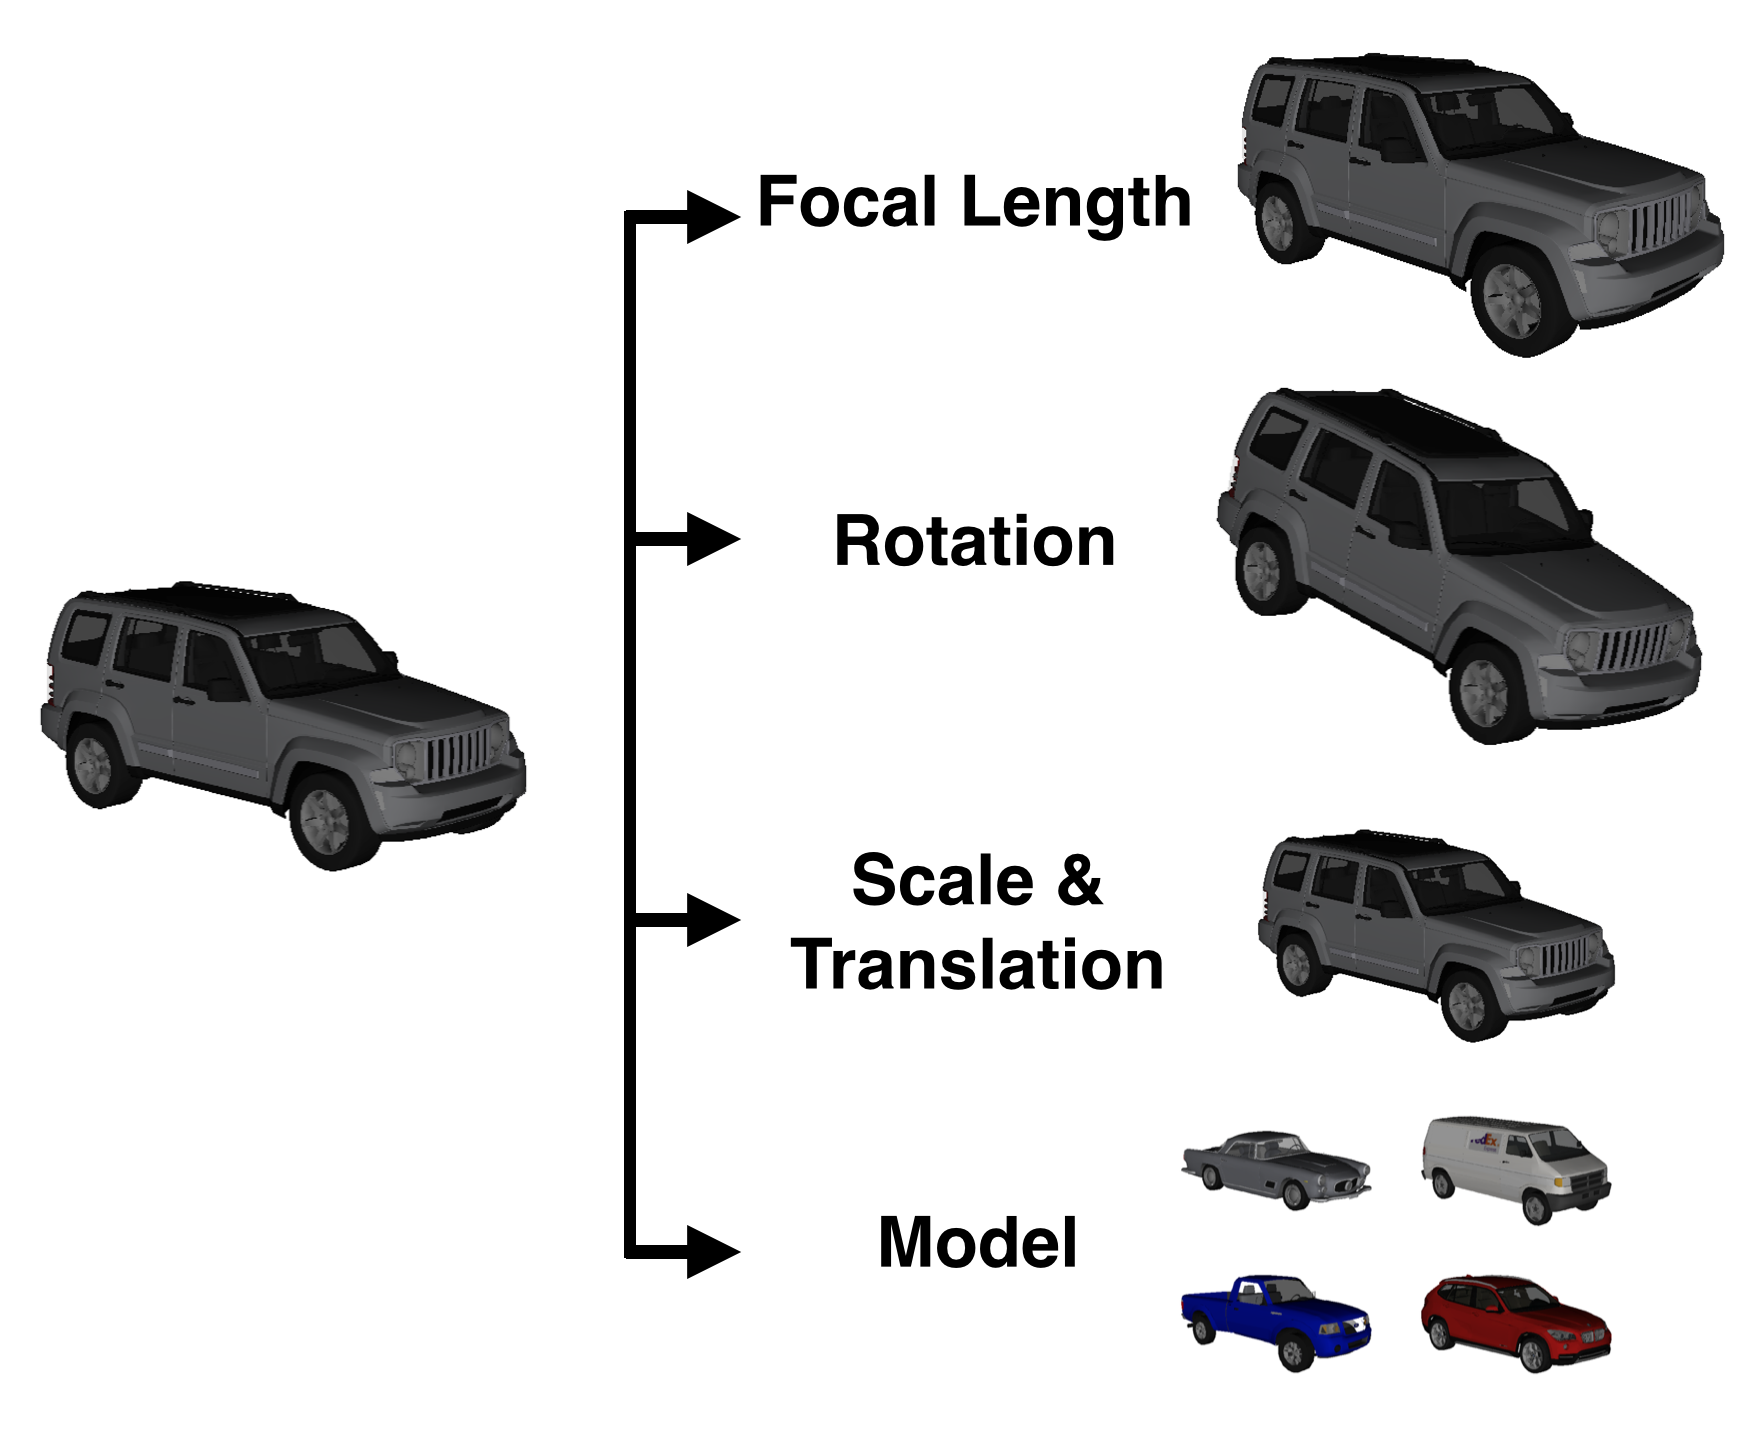
\includegraphics[width=0.7\linewidth]{tuning2} \\ [-5pt]
    \caption{Metropolis Hastings move types that are handled in fine-tuning stage (Section~\ref{sec:fine}).}
 \label{fig:moves}
\end{figure}


\paragraph{Initialization.}
Since the Metropolis-Hastings algorithm is susceptible to getting
stuck in local optima, we need a good initialization in order to
increase the probability to find a solution that is close to the
global optima. We achieve this by first running a discrete,
pre-trained version of our algorithm (i.e., an ensemble of NZ-WHO
templates) in order to get promising candidate 2D bounding boxes and
poses to start from. We then initialize $x_0$ for each of these candidates.
